\chapter{Literature Review}\label{C:review}

In this chapter, we first introduce the background of web service composition in Section \ref{overview}.  Followed that Section \ref{} discuss the single-objective service composition for both EC and non-EC based approaches. Section  \ref{} reviews existing works in muti-objective approaches and many-objective approaches.  Dynamic web service composition is covered in Section \ref{}. Section \ref{}  discussed most AI planning-based approaches to semantic service composition. Lastly, Section \ref{} summarises some critical points discussed in this chapter as well as some inadequacies or limitations in the literature review. 
\section{Semantic Web Service}\label{sevice}


Herein we utilise the formal definition from \cite{agarwal2010d5} to describe web service semantically: \textbf{a labelled transition system (LTS)}. A labeled transition system $L = (S,T,\rightarrow)$ comprises a set $S$ of states, a set $T$ of transition labels and a labeled transition relation $\rightarrow \subseteq S \times T \times S$. This transition system is established to present the actual behaviour of web services, which consists of a series of states. 

\begin{figure}
\centerline{
\fbox{
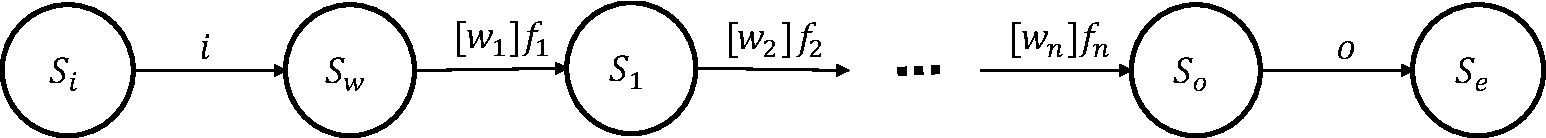
\includegraphics[width=14cm]{LTS.pdf}
}}
\caption{ The functionality of a Web Service \cite{agarwal2010d5}.}
\label{fig:lts}
\end{figure}


\begin{enumerate}

\item $S_i$ Start state includes knowledge available to web service before the web service is invoked by inputs; 
\item $S_w$ state includes the input parameters additional to the knowledge in (1); 
\item A series of state $S_1$ to $S_n$ proceed with corresponding actions $f_n$ that only occurred if each related condition $[w_i]$ is approved to be true. 
\item $S_o$ state contains all the output parameters. 
\item $S_e$ is the end state.  The four properties in the proposed web service model are inputs, state after input, state before outputs, and outputs. 
\end{enumerate}



To distinguish the changes between the pre-state and post-state, we model these changes using property instances. For example, inputs and outputs assigned with variable names and further referenced in pre and postcondition can be distinguished as instances from those exist in provider's knowledge bases. Therefore, the precondition using logic formula is assigned to the description of requirements of inputs( input types, relationships among them, or conditions on the value ) and conditions that must hold in the state after inputs. Similarly, the postcondition is restricted to the description of constraints on returned output, relationships between inputs and outputs, and changes caused by the service in service providers' knowledge bases. In the second model of the service request, it is expressed by logic expressions where both constraints on the nonfunctional property and functional property are also taken into account interpreted as A-Box statement.





\section{Web Service Composition}\label{overview}

Since one atomic web service could not satisfy or fully satisfy users' complex requirements, web service composition is approached by composing web services together with more sophisticated functionalities to meet the demand. Due to fully human intervention in manual service composition, so it is very time-consuming and less productive. Therefore, many approaches have been developed to achieve semi-automated or fully automated service composition. The semi-automated service composition is inspired by the business process that required prior knowledge to build up the abstract workflow. This workflow can be decomposed into several functional services slots for proper services being fitted. These steps are further discussed in Subsection \ref{lifecycle}. On the other hand, when we are composing services, both semi-automated and fully automated web service composition holds the challenge in the interoperability of services discussed previously. In particular, several problems are simultaneously taken into account. That is I/O matchmaking (i.e., the mechanisms of services for ensuring the interoperability ), discovery relevant services to the optimising the quality of service composition, e.g., overall QoS. Consequently, the following concerns are required to consider in generating composition solution. 


\subsection{Web Service Composition Lifecycle}\label{lifecycle}
Typical steps in a workflow-based automated Web service composition solution are shown in Fig. \ref{fig:lifecycle}. The detail of the service lifecycle is discussed as follows:

\begin{figure}
\centerline{
\fbox{
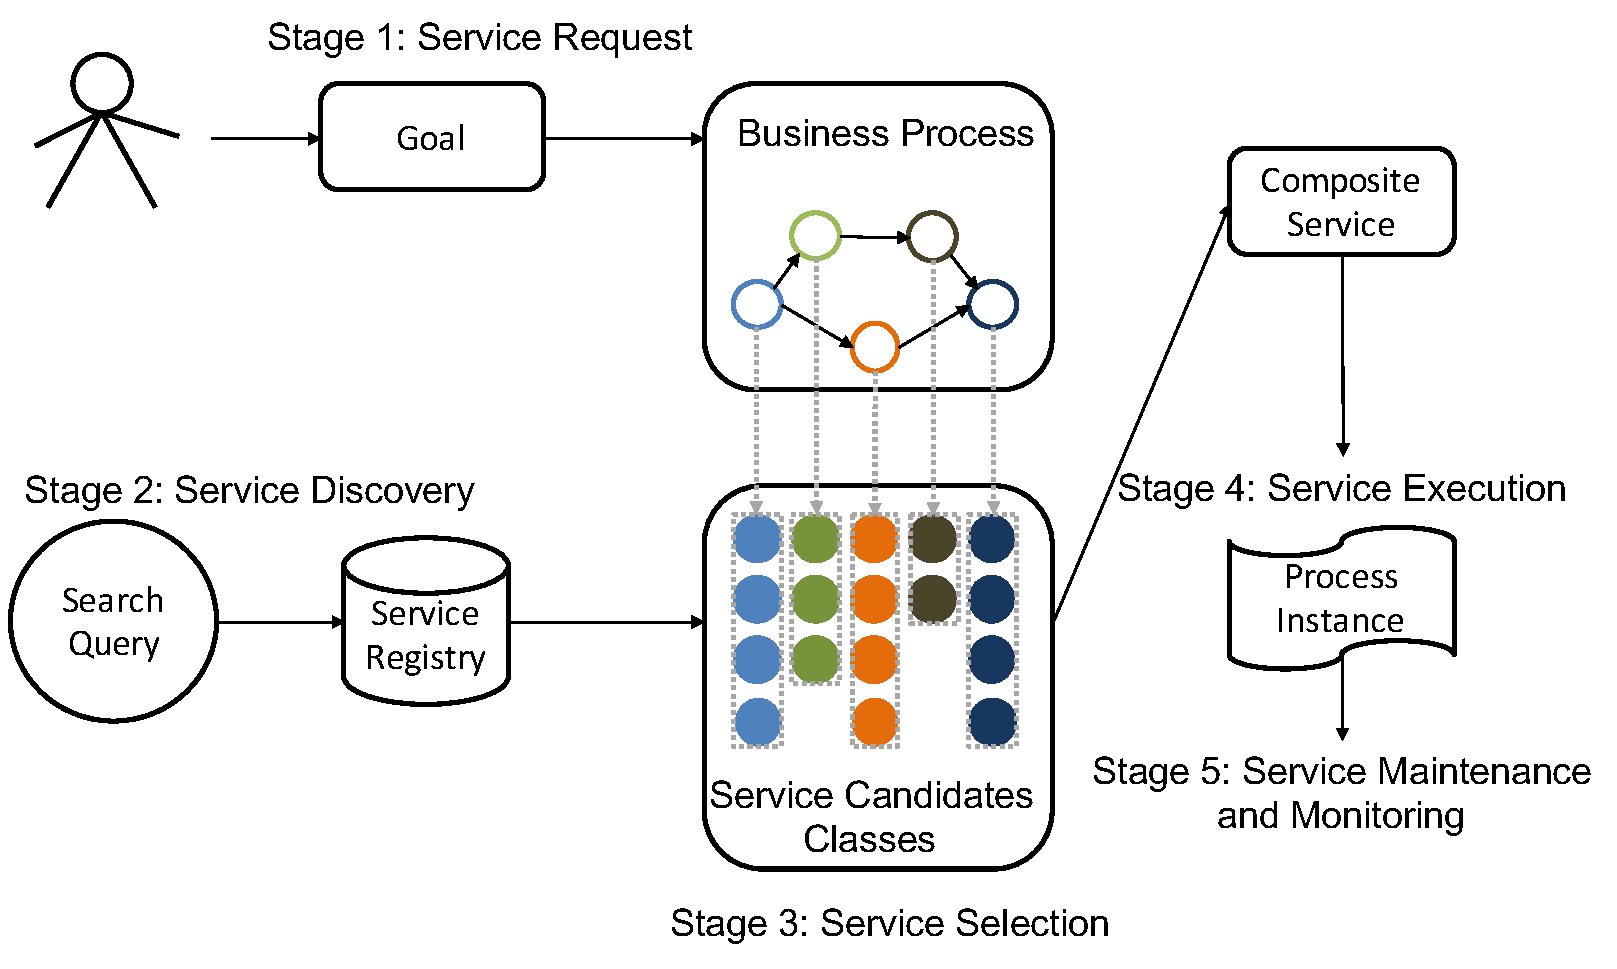
\includegraphics[width=14cm]{compositionLifecycle.pdf}
}}
\caption{ Web service composition lifecycle \cite{moghaddam2014service}.}
\label{fig:lifecycle}
\end{figure}

\begin{enumerate}
 \item \textit{Goal specification:} The first step in service composition is to collect users' requirements for composition goal that comprises of the functional (i.e., correct data flow ) and non-functional side (i.e., QoS). This step is achieved by building up an abstract workflow including a series of tasks with clearly defined functionality. Those tasks could be completed by selecting proper concrete services to reach desired QoS. 
 \item \textit{Service discovery:} Once the goal is clearly specified, concrete web services are to be selected for each task regarding its functional requirement. Often, more than one concrete web service is likely to be found to match the one task. However,  those matched web services are always different in QoS.  Therefore, web services are classified by the functionality of each task, i.e., inputs and outputs.
 \item \textit{Service selection:} At this stage, many techniques have been studied to select web services to best match each task for the satisfying functional requirement of each task and overall business process. Therefore, a plan of service composition is created ahead of execution.

 \item \textit{Service execution:} the process instance is monitored for any changes or services failures during service execution. In this stage, some actions are to be taken for adapting the changes.
\end{enumerate}
The web service lifecycle discussed above is a typical \emph{semi-automated approach}. There is a distinction between semi-automated and fully automated approaches. On the one hand, during the goal specification stage of semi-automated approach, the abstract work is already provided.  On the other hand, an abstract workflow is not provided at the stage of goal specification for \emph{fully automated service composition}. Often, fully automated service composition rely on some algorithms (e.g., Graphplan algorithm \cite{blum1997fast}) to achieve service composition, during which service workflow is gradually built up along with the service discovery and service selection at the same time. In this proposal, I concentrate on developing methods for fully automated service composition since it has been shown the flexibility. Also, herein service discovery and service selection are considered as interrelated tasks that are interleaved with the composition algorithm.


\subsection{I/O Matchmaking}\label{matchmaking}
\subsection{Service Discovery}\label{servicediscovery}
\cite{agarwal2009d5} discussed three mechanisms of semantic web service discovery: classification-based approach, functionality-based approach and hybrid approach. The first one makes use of the classes provided by WSMO-Lite language for service semantic annotation so that service requesters can use class names to express a goal offering a straightforward discovery from a set of classes. However, classes without meaning association could lead to the incomprehensibility of web service discovery.  The second one does not take classes into account, but consider functional aspects of web service including pre and postconditions. The actual functional description of web service is defined as a tuple consisting input, output, precondition and postcondition where optional variables or constants described by postcondition are only satisfied if the conditions are held in the knowledge base by precondition. The desired function is also defined and revealed the differences between the actual and desired functional description. The project also developed a discovery algorithm to handle different input, output, precondition and postcondition with associated concepts and relations in the provided domain knowledge base. The key idea of the matching is to check for the satisfiability of implications that actual precondition and actual postcondition must imply the desired precondition and desired postcondition respectively.  The strength of the second is that it potentially meet the demands of all the comprehensible discovery while the weakness of that lacks efficiency and scalability. The third approach is based on classification and functionality-based discovery. Classification hierarchy is proposed to achieve automatic semantic reasoning in hierarchical functionality with consideration inconsistency. Therefore, the definition of overall inputs, outputs, precondition and postcondition of a functionality class are determined to fulfil consistency of hierarchical classes formally if the precondition, postcondition, inputs and outputs of the subclass in conjunction with the overall precondition, postcondition inputs and outputs of the super class. The discovery of the third approach is to find a query against the hierarchical functionalities. The advantage of this approach is to achieve better performance combining strengths of the previous two pure classifications based and functionality based approaches. While the classification hierarchy needs to be kept consistent when a new web service is published or updated, which is very time-consuming in computation.​


\subsection{Composition Optimisation}\label{matchmaking}


%Besides identifying the atomic Web services most suitable to fulfilling key composition tasks, the selection process often takes additional user constraints into account. A survey of the literature in the area shows that two types of contraints are commonly taken into account. The first group comprises the creation of service compositions that are optimised according to the Quality of Service (QoS) constraints on its constituent atomic services, where QoS attributes may be thought of as features that indicate the quality of a given Web service, such as the time it requires to return a response and its financial cost of execution \cite{da2014graph}. The majority of works in this area use maximising and minimising functions for the different QoS attributes, meaning that they attempt to obtain solutions with the best possible qualities without any thresholds \cite{wang2013improved,parejo2008qos,yoo2008web,garcia2008qos,zhang2010qos,wang2012survey,moghaddam2014service,kattepur2013qos,DBLP:journals/soca/LiZDSGL13}. However, there also exist approaches focused on what may be referred to as a Service Level Agreement (SLA)-aware optimisation, which is solutions must meet certain predetermined QoS thresholds in order to be considered valid (e.g. the financial cost of each service used in a composition must not exceed 50 dollars) \cite{yoo2008web,yin2014hybrid,chen2014partial,berg2013revenue}.

%The second group comprises the creation of service compositions that have multiple execution branches, indicating user preferences at runtime \cite{wang2014automated,boustil2010web,karakoc2009composing,marconi2006specifying,bertoli2009control}. For example, the output of a service \textit{A} determines which service to execute next; if the output is greater than a certain threshold, then service \textit{B} should be executed; otherwise, service \textit{C} should be executed instead. These preferences are expressed logically as conditions, and affect the workflow used to establish the connections between services rather than the individual services themselves. These two types of user constraints are discussed in more detail in subsequent Sections in this chapter.

%\subsection{Web Service Composition in Practice}

%The research material published on Web service composition is highly theoretical and frequently employs layers of abstractions and simplifications intended to make the problem at hand manageable. However, it is also important to investigate how these ideas fit into practice, which is the objective of this Subsection. As mentioned earlier, while significant amounts of work are being performed in the field of automated Web service composition, these approaches ultimately remain on the theoretical level due to difficulties that have not yet been fully addressed. On the one hand, a study \cite{lu2007web} has shown that the composition of services is fraught with issues. A central problem is that there are discrepancies between the concepts used by different services: the schemas used differ from each other, even if the services handle exactly the same domain. Another problem is the existence of services that produce too much data, low-quality data, or that incur too much latency. These characteristics may slow down the execution of the composition and even require human intervention, defeating automation efforts.

%On the other hand, an automated framework for Web service compositions which can be applied to real services has already been proposed \cite{marconi2007automatedweb}.
%The functionality of this framework was demonstrated by creating a composition that uses the Amazon Virtual Cart service, the Amazon
%Book Search service and a bank's Point of Sale Web service. The authors of the framework point out that it is very challenging to find service documentation that is comprehensive enough, and that functionality details had to be identified from natural language explanations intended
%for developers who are working manually. Additionally, the specification of control flow requirements must be performed manually using a logic programming language. Despite these difficulties, the evaluation of this framework shows that a composition can be found within seconds when using it as opposed to an estimated 20 hours of manual development, showing that research on Web service composition provides some immediate benefits.

%These two works provide opposing views on the viability of automated Web service composition, however a more recent approach \cite{mobedpour2013user} presents the interesting middle ground of user-centered design. This systems combines manual and automated techniques, providing a browsing tool that allows users to explore the repository and gain some understanding of the offered QoS value ranges of services before having to write any QoS requirements, as users may often be unaware of what a reasonable QoS value would be for a given dataset. Users are also supported through the selection process by utilising a UI that diminishes their cognitive overload, and helps them express their requirements using a standardised language. In addition to these tools, this approach also proposes a clustering algorithm that groups service candidates according to their range of QoS values, with the objective of providing selection options when users have fuzzy (i.e. soft) requirements. The strength of this approach is that it does not undervalue human intervention in the composition process, instead providing tools that empower system users. As Web service composition always requires some degree of user involvement, at the very least when setting composition requirements, this type of approach may prove to become an increasingly popular composition solution.

%\section{Single-Objective QoS-Aware Composition Approaches}\label{SingleObjective}

%This section discusses composition approaches that optimise solutions according to their overall QoS. These approaches can be divided into biologically inspired methods, which use Evolutionary Computation to reach their goal, ang general optimisation approaches that do not turn to evolutionary techniques. These two groups are quite distinct, but they have the commonality of using an objective function as the guide with which to measure the quality of the candidate solutions.

%\subsection{Biologically-Inspired Approaches}

%Biologically-inspired Web service composition approaches rely on evolutionary computation algorithms, which implement their search strategies by drawing inspiration from nature, namely the behaviour of social animals such as bees, fish, and ants. An important distinction between these different bio-inspired approaches is in their representations of the composition problem. These varying representations are discussed throughout this Subsection, and visually summarised in figure \ref{fig:representations}. \textbf{Genetic Algorithms (GA)} are a popular choice for tackling combinatorial optimisation problems, and thus have been widely applied to the problem of Web service composition \cite{wang2012survey}. The encoding scheme for a composition is commonly done as a vector of integers, where each integer corresponds to a candidate Web service, even though some authors have attempted to use matrix representations that also include semantic information about services. A population of candidates is evolved for several generations using generic operators, typically crossover and mutation: in crossover, equivalent sections of the vectors in two distinct candidates are swapped; in mutation, a section of one candidate's crossover is modified at random in order to introduce some genetic diversity. An observed problem with the GA technique is that it tends to prematurely converge to solutions, thus preventing the exploration of further possibilities. \textbf{Particle Swarm Optimisation (PSO)} bears similarities with GA, also relying a on vector representation for candidates. However, instead of employing genetic operators to carry out the search process, PSO uses the concept of position updates to move candidate particles across the search space. As PSO may also present the problem of not fully optimising solutions (i.e. converging prematurely), hybrid approaches have been attempted to improve its efficiency and optimisation power \cite{wang2012survey}. A key limitation of both GA and PSO is in the underlying vector representation used by candidates, since it makes it very challenging to encode workflow information and thus perform any type of fully automated Web service composition.

%\begin{figure}
%\centerline{
%\fbox{
%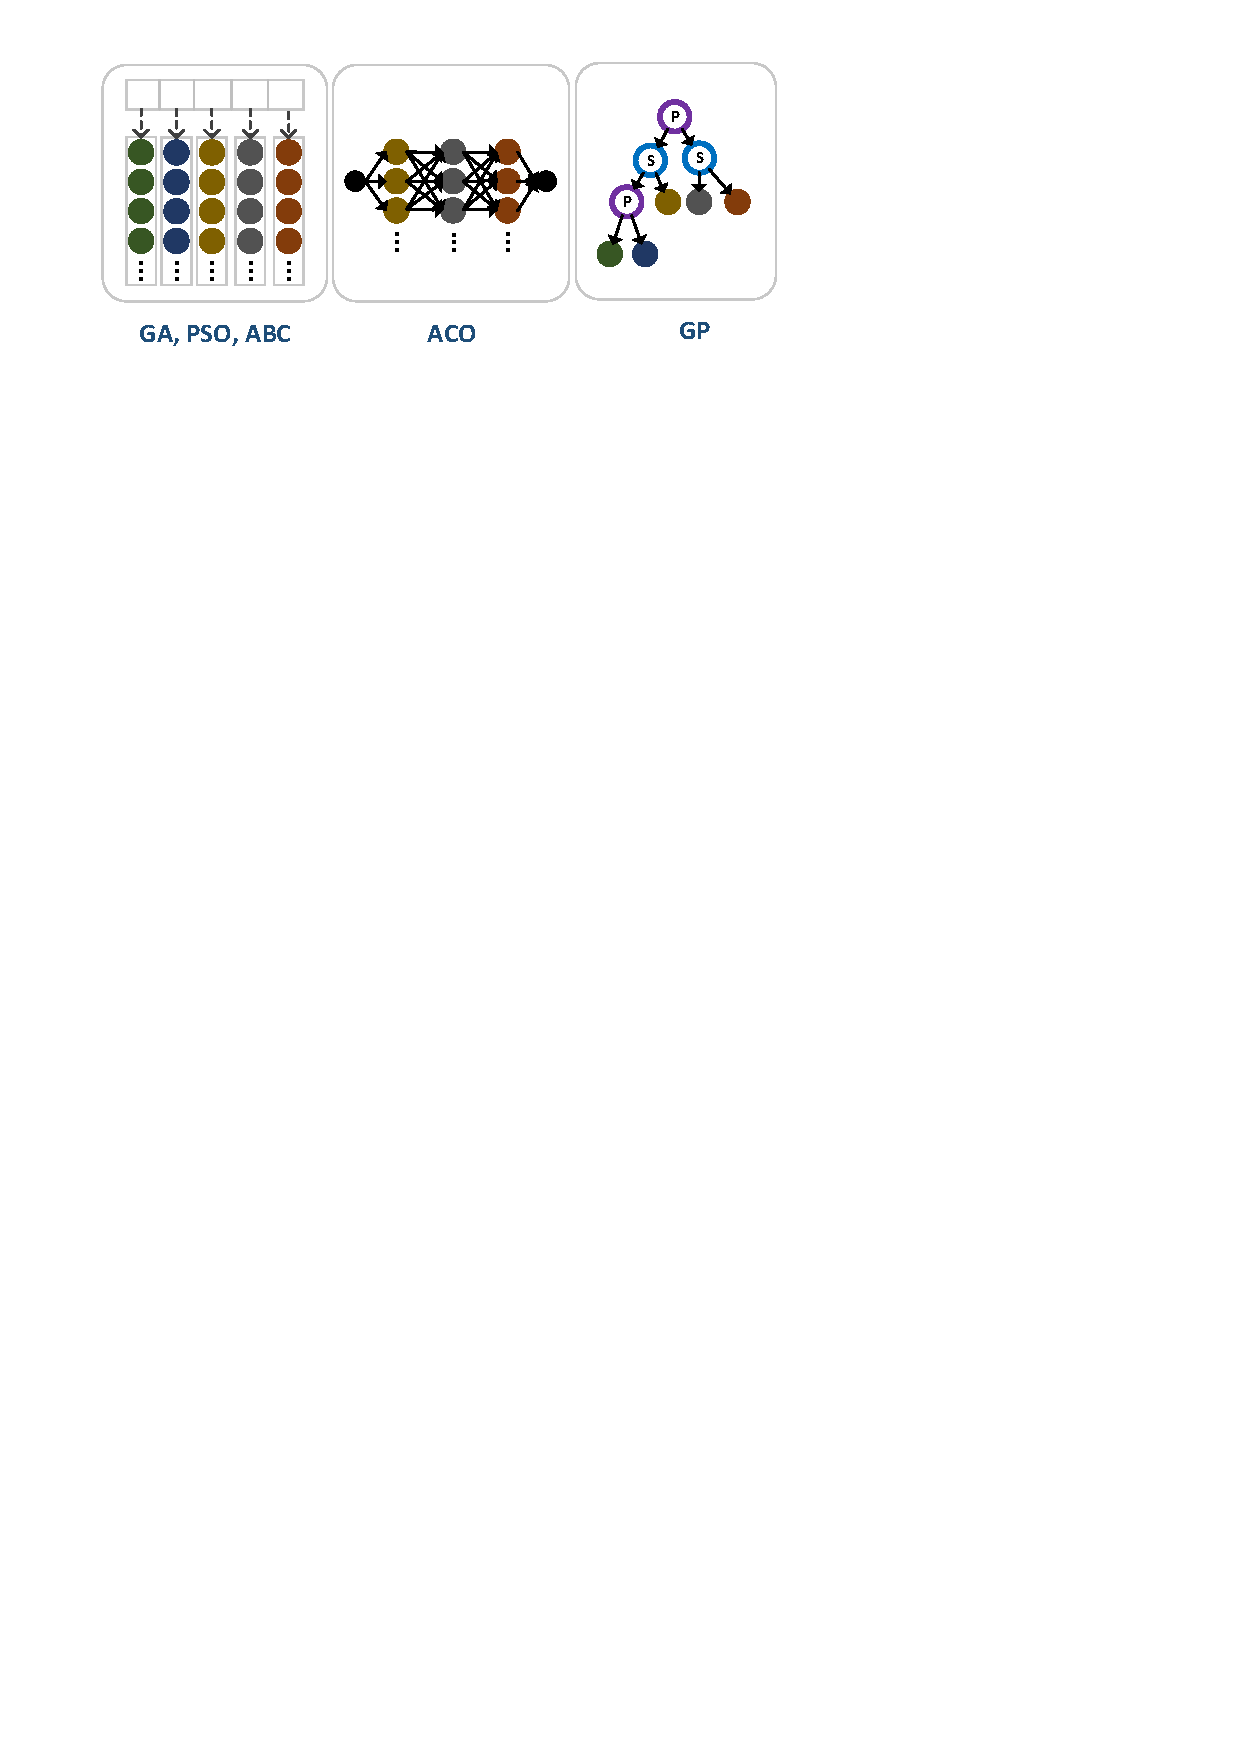
\includegraphics[width=14cm]{representations.pdf}
%}}
%\caption{The different problem representations employed by biologically-inspired Web service composition approaches.}
%\label{fig:representations}
%\end{figure}

%\textbf{Ant Colony Optimisation (ACO)} has also been proposed as a solution to QoS-aware Web service composition \cite{zhang2010qos}. ACO is particularly suitable to a directed acyclic graph (DAG) representation, in other words, the workflow composition representation commonly used in the field. In ACO, the Web service workflow is built to be traversed by a group of ants (agents). At each fork in the graph, the ants choose which path to follow based on probabilities that take into account the strength of the pheromones left by other ants, and also a heuristic function for that particular graph. The pheromones left by the ants are updated after all ants have toured through the graph once, with paths of higher fitness resulting in a larger pheromone increment for the edges of those paths. Meanwhile, the pheromone level of all edges gradually decreases (i.e. evaporates) after each tour of the ants. The graph representation in this technique follows the abstract workflow idea, with a pool of concrete Web services associated to each abstract Web service. Each pool of candidates is a layer that is fully connected to the layers of any following abstract services, so that an optimal path can be chosen from the edges laid out. For each concrete Web service, the heuristic factor is calculated based on its QoS values, and the fitness function also measures QoS attributes. As with GA and PSO, this representation also amounts to the idea of semi-automated Web service composition, even though in this case the encoding of workflow information leading to a fully-automated approach would seem to be trivial.

%The works in \cite{zhang2010qos} and \cite{wang2013improved} apply the \textbf{Artificial Bee Colony (ABC)} algorithm to Web service composition. The ABC algorithm simulates the behaviour of bees search for food sources. The position of food corresponds to candidate solutions in the search space, encoded as a service vector, and there are three types of bees dedicated to searching: \textit{Employed bees} exploit the neighbourhood of a single food source already found; \textit{Onlooker bees} exploit the neighbourhood of different food sources depending on the dance behaviour displayed by employed bees; \textit{Scout bees} are the bees sent to random food sources after the neighbourhood they were previously exploiting does not present any food sources that are better than the original. The roles of the bees change according to the colony's needs, which is a feature unique to this algorithm. One of the issues with this approach, as pointed out by the authors, is the search space it explores. The problem with the typical search space for Web service composition is that it is organised based on the proximity of the components included into the composition. For example, given two adjacent solutions $a$ and $b$ in the search space, $a$ will only have one service that is different from all the services included in $b$. Despite being neighbours, however, the fitness values of $a$ and $b$ may be radically different, and as the optimisation occurs according to a fitness function, this means that the search space is not entirely continuous. These works modify the traditional ABC algorithm to take this problem into account, filtering the neighbourhood of each solution during the search and excluding radically different neighbours from consideration.

%\textbf{Genetic Programming (GP)} is, from this project's perspective, possibly the most interesting technique for the problem of Web service composition. That is because GP, unlike the previously discussed techniques, is capable of supporting fully automated Web service composition. In GP approaches \cite{aversano2006genetic,rodriguez2010composition}, workflow constructs are typically represented as the GP tree's non-terminal tree nodes while atomic Web service are represented as the terminal nodes. In this context, workflow constructs represent the output-input connections between two services. For example, if two services are sequentially connected, so that output of service \textit{A} is used as the input of service \textit{B}, this would be represented by a sequence workflow construct having \textit{A} as the left child and \textit{B} as the right one. The initial population may be created randomly, in which case the initial compositions represented in that generation are very unlikely to be executable due to their mismatched inputs and outputs, or it may be created using an algorithm that restricts the tree structure configurations allowed in the tree to feasible solutions only. A fitness function is employed for the QoS optimisation of candidates, and the genetic operators employed for this evolutionary process are crossover, where two subtrees from two individuals are randomly selected and swapped, and mutation, where a subtree for an individual is replaced with a randomly generated substitute. One of the difficulties of tackling the problem of Web service composition using GP is that it does not intrinsically support the use of constraints \cite{craenen2001handle}, meaning that even if all candidates in a population meet the feasibility constraints, there is no guarantee that subsequent generations will maintain conformance to them. The approaches discussed above handle this problem in one of two ways: by \textit{indirect constraint handling}, where feasibility constraints are incorporated into the fitness function so that the optimal function value reflects the satisfaction of all constraints, or by \textit{direct constraint handling}, where the basic GP algorithm is adapted at the initialisation and genetic operation stages to ensure that the feasibility constraints are met. Indeed, the tree representation of an underlying workflow composition may pose difficulties whenever constraint verification is necessary.

%\subsubsection{Graph Variations of GP}

%Genetic programming using candidates constructed as graphs (instead of trees) would be ideal for the problem of Web service composition, since dependencies between services could be intuitively encoded. Even though variations of GP with graph candidates do exist, they have not been employed in this domain, therefore the focus of this section is on the techniques and not on the composition problem. Galvan-Lopez \cite{galvan2008efficient} proposes a general-purpose EC technique that is modification of the usual GP tree reprentation, allowing the creation of graphs. The key extension proposed here is the addition of pointer functions to certain non-terminal nodes, meaning that they can have connections to nodes in independent subtrees. Program inputs are provided as terminal nodes (similarly to the output-as-root representation discussed earlier), but instead of having a single output location at the root node, they may have other output locations as well, inserted as necessary amongst the non-terminal nodes of the tree. Since the overall tree structure is maintained, it becomes possible to perform the crossover and mutation operations similarly to their implementation in the case of a simple tree. The main difference is that any pointers present in the original tree may not be modified when these operations are applied. In order to ensure that the number of outputs in a tree remains correct throughout these genetic operations, each node in a tree is classified beforehand to establish which ones may be selected for the crossover operation. This representation makes it easier to evolve graphs, however it does not support strongly-typed GP, which is of interest to our research. In addition, each tree is still required to have a single root, meaning that there are connections between the different output nodes. In our problem domain, this is a hindrance because the output nodes must be completely independent from each other.

%Miller and Thomson \cite{miller2000cartesian} present Cartesian Genetic Programming (CGP), a popular technique for evolving graph structures. The simplicity of SGP lies in the fact that it can represent the genotype of candidates as a string of fixed length, meaning that crossover and mutation operations are trivial to implement provided that they obey some simple constraints. The core idea of CGP is to create a two-dimensional array of programmable nodes of a predefined size. Each node has a predefined number of outputs, and the overall array has a predefined number of inputs and outputs. Then, as this structure is evolved, the functions inside of each node can be reprogrammed, and so can the inputs those nodes require. From that point onward, the structure can be optimised according to the algorithm's fitness function. One important observation is that CGP may have unexpressed genes, meaning that not all the nodes in the two-dimensional array are necessarily components of the final answer. One limitation of this approach is that CGP does not easily handle strongly-typed GP, thus restricting the range of problems it can be applied to. Another problem is that it requires predefined numbers of nodes and node inputs/outputs, making it difficult to represent compositions with varying numbers of services and service inputs/outputs.

%Mabu, Hirasawa and Hu \cite{mabu2007graph} introduce a technique for the evolution of graph-based candidates, called Genetic Network Programming (GNP). GNP has a fixed number of nodes within its structure, categorised either as processing nodes (responsible for processing data) or as judgment nodes (perform conditional branching decisions), and works by evolving the connections between these fixed nodes. Connections are represented in a linear gene structure, and the number of outgoing connections from a node is dependent on the type of that node: processing nodes have a single outgoing connection, while judging nodes have more than one (depending on the number of branches desired). Because of the linear representation of connections between nodes, the genetic operators employed for the evolutionary process are quite simple. The mutation operator randomly chooses the destination of a node's outgoing connection; the crossover operator swaps two nodes with the same label from two different solutions, taking their outgoing edges with them. Li, Yang and Hirasawa \cite{li2014evolving} extend the basic GNP idea by using the Artificial Bee Colony (ABC) approach to evolve candidates. While these approaches present the advantage of simple genetic operations, the number of nodes and outgoing edges per node must be fixed throughout the evolutionary process, meaning that it suffers from the same limitations discussed above.

%Poli \cite{poli1996parallel} presents an EC algorithm where solutions are represented directly as graphs. This graph is mapped to a grid, where each row represents a layer of the graph, and columns can be used freely to accommodate the nodes in a layer. By using this representation, it is possible to perform relatively simple mutation and crossover operations to a graph without compromising its syntactic correctness. For the crossover operation, a crossover point (node) is selected in each candidate, and all the ancestors of that node are identified. These two subgraphs of ancestors are then swapped, a process that may overwrite nodes from the other graph but that maintains any original edges. Whenever this swap causes parts of the subgraphs to be placed outside of the grid, these nodes are "wrapped around" their respective rows, meaning that they are moved to the other extreme of the row. For the mutation operator, an existing subgraph is selected and replaced with a newly created one, using the same general mechanism as the crossover. Once again, while this approach makes the implementation of genetic operations simple, it does not allow for correctness constraints (i.e. input-ouput connections) to be maintained. Additionally, this representation assumes that the duplication of nodes is acceptable, which may pose some problems in the domain of Web service composition.

%Kantschik and Banzhaf \cite{kantschik2002linear} propose linear-graph GP, a structure that allows programs with multiple execution paths to be optmimised using evolutionary computing. This approach is an extension of the simple linear program representation where each element of a vector contains one program instruction. In this representation, a program graph contains several nodes, and each of these nodes contains a portion of a linear program that may be executed according to preceding branching conditions. Within each of these nodes, there exists also a branching node that is responsible for determining which outgoing edge to follow (i.e. which execution path to choose after executing the current node). The branching functions contained in each of these nodes may read the values of variables manipulated in the linear program portion that is located in the same graph node. The mutation operator in this approach may alter an individual entry within a linear program vector, the branching function within a branching node, or the number of outgoing edges of a given graph node; the crossover operator may exchange individual entries within linear vectors of two candidates, or exchange a group of contiguous graph nodes between two graphs. Despite allowing branching constructs, this approach is not useful to our research because non-sequential relationships between different Web services cannot be encoded into linear representations.

%The works in \cite{globus1999automatic,brown2004graph,nicolaou2009novo} present a graph-based genetic algorithm that is used to evolve representations of molecules. Atoms are represented as nodes, and their bonds as edges. Two types of genetic operations are supported: mutation, which can be the appending or removing of a node and its connecting bonds,
%and crossover, where edges are removed from each candidate until each graph is divided into two disconnected subgraphs that are then reconnected to create new child candidates. The reason why these genetic operators can be used without compromising the strucuture of the molecule is that the only restriction when creating a new connection is the valence of a given atom (i.e. the number of bonds it can make), but bonds do not need to be directed edges and cyclic structures are allowed. In the Web service composition domain, however, the need for additional restrictions means that these genetic operators are no longer suitable.

%\subsection{Other Optimised Composition Approaches}

%Other methods exist for producing optimised Web service composition results in addition to biologically inspired approaches, and a subset of them is presented in this section. \textbf{Tabu search} \cite{glover1989tabu} is a combinatorial optimisation strategy for identifying an optimised solution amongst a group of candidates, typically in problems where exhaustive search is prohibitively expensive. In Tabu search, an objective function (either linear or nonlinear) is used to measure the goodness of solutions, encouraging solutions with the least penalty (i.e. optimal solutions). Then, a range of moves that lead from one candidate solution to another is defined. For a particular candidate solution,
%there is a set of moves that can be applied to it, and this is known as the neighbourhood function. One of the biggest advantages of Tabu search is that, unlike the
%hill climbing technique, it can avoid being stuck at local optima when searching. The technique keeps track of a set of tabu moves, which are moves that violate a given
%collection of tabu conditions. The objective of having a tabu set is to prevent the search from reaching solutions whose best next move has already been visited (i.e. prevent cyclic search moves). Due to its relative simplicity and its flexibility of implementation, tabu search has a wide range of practical applications for combinatorial
%optimisation problems. For example, a technique that combines Tabu search and a hybrid Genetic Algorithm (GA) implementation has been proposed recently \cite{parejo2008qos}. For the Tabu search component of the technique, a move is defined as a change in one of the concrete services used as the solution, and the Tabu set is a fixed-size set of the latest
%\textit{n} solutions visited. For the hybrid GA, the same basic idea of the traditional GA is applied (set candidate sizes, two-point crossover, mutation that randomly chooses another concrete service), however a local improver is also employed. This improvement process randomly explores a percentage of a solution's neighbourhood. A drawback of using Tabu search for Web service composition is that the structure used for the representation of candidates is typically linear \cite{parejo2008qos,bahadori2009optimal}, which restricts the problem model to address semi-automated compositions only.

%\textbf{Integer Linear Programming (ILP)} has also been applied to composing Web services \cite{yoo2008web}. ILP is flexible in the way it represents problems, therefore a fully automated Web service composition approach that also takes non-functional attributes into account when constructing the best solution can be solved using it. An objective function is defined for the achieving the optimal QoS values, and several other functions are used to restrict the functionality of the solutions (i.e. restrict the search space). For linear programming, we first determine the "corners" of the restricted search space (i.e. where two constraint lines meet), and then apply the objective function to each of these solutions. One of these "corner" solutions is the optimal one, provided that all boundary functions are linear, so the best objective function score indicates the final solution. While ILP applied to Web service compositions is guaranteed to find an optimal solution, it has been shown to be very inefficient in comparison to EC-based approach as the complexity of the problem increases \cite{aversano2006genetic}. Another problem with the ILP approach is that it is likely to pose difficulties when used for creating compositions with multiple execution paths, as branching constraints would have to be represented using a linear function.

%\textbf{Structural Equation Modelling (SEM)}, a statistical analysis method for forecasting values according to current measurements, has been used in a service selection strategy that considers the future trends of the QoS values of the candidate services \cite{DBLP:journals/soca/LiZDSGL13} as opposed to relying on static QoS snapshots. By being able to predict the QoS trends of services, it is possible to create a composition that is optimal at execution time. One key advantage of SEM is that it is capable of accommodating changes in the user preferences (weights) associated with each QoS attribute, and can use the errors in QoS measurement histories to create a forecast model. The proposed approach was tested using different composition algorithms (e.g. ILP) enhanced with SEM, with a dataset that simulates the changes of QoS parameters over time. Results show that the prediction model for QoS values is initially quite inaccurate, but the accuracy increases for both algorithms as days go by and a history of values is built. While this method is very effective at predicting QoS values to aid in the optimisation of solutions, it cannot be used alone to compose Web services. Thus, SEM is not considered further in this work.

%Finally, \textbf{Algebraic Expressions (AE)} have been employed to the problem of Web service composition \cite{ferrara2004web, kattepur2013qos}. A formal representation of a Web service composition is used in this approach, relying on algebraic constructs to describe the behaviour of atomic Web services and to constraint the characteristics of a correct composition solution. One of the main advantages of AE is that this technique is expressive enough to emulate the behaviour of Web service composition languages such as BPEL4WS, thus it is possible to design and verify composition solutions entirely through AE. A more flexible composition option, explored in \cite{ferrara2004web}, involves constructing a mapping between algebraic expression and BPEL, to allow for an automated translation between these two representations. The work in \cite{kattepur2013qos} goes further, proposing a composition algorithm that also performs QoS optimisation based on algebraic expressions. Despite promising, the disadvantage of this technique is that it requires the composition task to be described in formal terms that are challenges to system users without the necessary background.

\section{Multi-objective, and Many-objective Composition Approaches}\label{MultiObjective}

%\begin{equation}
%fitness_i = w_1A_i + w_2R_i + w_3(1 - T_i) + w_4(1 - C_i)
%\end{equation}

%\centerline{where $\sum_{i=1}^{4} w_i = 1$}
%\vspace{0.7cm}
%----------------------chen starts---------------------------------------------------
Maximising or minimising a single objective function is a most commonly used way to handle optimising problems in automated web service composition.  That is a Simple Additive Weighting (SAW) \cite{hwang1981lecture} technique, which presents a utility function for all the individual quality criteria as a whole. This technique optimises and ranks each web service composition using a single value for each solution. However,  the limitation of this technique lies in not handing the conflicting quality criteria.  Those conflicting quality criteria are always presented trade-offs. To overcome this limitation, a set of objectives corresponding to different independent quality criteria are optimised independently. Consequently,  a set of promising solutions that present many quality criteria trade-offs are returned.


\subsection{Multi-objective approaches}\label{MultiObjective}

Many multi-objective techniques \cite{liu2005dynamic,zhang2010qos,yu2013efficient,yin2014hybrid,xiang2014qos,chen2014partial} have been investigated to extensively study QoS-aware web service composition problems.  A set of optimised solutions is ranked based on a set of independent objectives, i.e., different QoS attributes. In particular, solutions are compared according to their relationship for domination. Especially, figuring out solutions are clearly dominating the others. For example, given two service composition solutions that are compared based on execution cost $c$ and execution time $t$, solution one, $wsc_1(c=10,t=1)$ and solution two,  $wsc_2(c=13,t=1)$. In our context, $wsc_1$ dominate $wsc_2$ as $wsc_1$ has the same execution time and a lower execution cost. If given $wsc_3(c=10,t=2)$, $wsc_2$ is a \textit{non-dominant} solution in the relation to $wsc_3$ because of its longer execution time and cheaper execution cost. Therefore,  If those non-dominant solutions are globally produced among both the dominant and non-dominant solutions, i.e., they do not dominate themselves. These solutions are called a \textit{Pareto front}, which provide a set of non-dominant solutions for users to choose.


\subsubsection{Multi-objective techniques with GA} Many approaches to multi-objective Web service employs GA \cite{liu2005dynamic}, but other EC algorithms are also considered. For GA, \cite{liu2005dynamic} employs a service composition model, called  MCOOP (i.e., muti-constraint and multi-objective optimal path) as web service composition solution for only a sequence service composition considered in the paper. In this model, different paths are selected from a service composition graph that includes $N$ service group. In each group,  services present same functionality with different QoS.  Apart from that, GPDSS is proposed to generate the outputs of Pareto optimal composition paths. In particular, two points crossover and mutation are applied to speed up the astringency of this algorithm. The work \cite{wada2012e3} investigates a semi-automated approach to SLA-aware web service composition problem.  Each linear representation proposed here presents three service composition solutions designed for three group users' categories.  The individuals are randomly initialised, evaluated and optimised with objectives from all the possible combinations of throughput, latency, cost and user category.  In this work, two multi-objective genetic algorithms: E-MOGA and Extreme-E are developed. E-MOGA is proposed to search a set of solutions that equally distributed in the searching space by the means of fitness function, where the production of domination value,  Manhattan distance to the worst point and sparsity (i.e, Manhattan distance to the closest neighbour individual)  is assigned to the feasible individual as fitness value, and SLA violation /domination value is assigned to the infeasible solutions. On the other hand, Extrem-E provide extreme solutions by employing fitness functional, where weights use a term 1/exp(p-1), where $p$ is the number of objectives and is assigned to the $p^{th}$ objective.

\subsubsection{Multi-objective techniques with PSO} The work \cite{yin2014hybrid} combines genetic operators and particle swarm optimisation algorithm together to tackle the multi-objective SLA-aware web service composition problems. The method proposed in the paper  is considered to be more effective in  considering different scare of cases.  It is called as HMDPSO, i.e., hybrid multi-objective discrete particle swarm optimisation. In particular, the updates of particle's velocity and position are achieved by the crossover operator, where both velocity and position of new individual are updated in accordance with positions of \textit{pbest}, \textit{gbest}, and current velocity. On the other hand, mutation strategy is introduced to increase the diversity of particle and is performed on the \textit{gbest} particle if the proposed swarm diversity indicator is below some value. For the evaluation,  the fitness values of individuals are assigned in the same way as the E-MOGA method in \cite{wada2012e3}.

\subsubsection{Multi-objective techniques with ACO} Generally, ACO simulates foraging behaviours of a group of ants for optimising the traversed foraging path, where the strength of pheromones is taken account for. The work \cite{zhang2010qos} turns the service composition problem into path selection problem for the given abstract workflow with different service candidate set.  It employs a different strategy of "divide and conquer`` for decomposing a given workflow. That is,  two or more abstract execution paths are decomposed from the workflow and have no overlapped abstract services. This decomposing strategy results in a much smaller length of the execution paths compared to those in the works \cite{yu2007efficient}.  Also, a new ACO algorithm is proposed to handle the multi-objective QoS-aware service composition problem. In particular,  the phenomenon is presented as a k-tuple for $k$ objectives, rather than a single value. Apart from that, a different phenomenon updating rule is proposed by considering an employment of a proposed utility function as a global criteron. The paper \cite{wang2014novel} introduces nonfunctional attributes of web services to include trust degree according to the execution log. Also, a novel adaptive ant colony optimisation algorithm is proposed to overcome the slow convergence presented from the traditional ant colony optimisation algorithmd. In particular, the pheromone strength coefficient is adjusted dynamically to control both the updating and evaporation of pheromone. The experiment results are analysed in an alternative way. That is, the total Pareto solutions are combined from different compared ACO algorithms, then the accurate rate of each algorithm is calculated based on the compared Pareto solutions identified in the total Pareto solutions. The results also show more Pareto solutions found compared to the traditional ACO methods. However, the experiment is only conducted for the evaluation of a small case study, where only a simple abstract workflow is studied.

\subsection{Many-objective approaches}\label{ManyObjective}

Herein, more than three objectives in Multi-objective problems (MOPs) are often considered as many-objective problems. Ishibuchi et al. \cite{ishibuchi2008evolutionary} present an analysis of the multi-objective algorithm for handling optimisation problems with more than 3 objectives. However, they address that the searching ability is deteriorating while the number of objectives is increasing, since the non-dominated solution is very large, which make it harder to move solutions towards the Pareto Front.

The work \cite{de2010many} employs NSGA-II to deal with five different quality criteria (i.e., runtime, price, reputation, availability and reliability) for semi-automated web service composition problem.  To examine the techniques to decrease the deterioration, two preference relations proposed by \cite{bentley1997finding} are applied to NSGA-II: Maximum Ranking (MR) and Average Ranking methods (AR). In particular, MR is the best of all the ranking scores from all the objectives, and AR is a sum of all the ranking scores from all the objectives. Therefore, three algorithms (NSGA-II, NSGA-II with MR and NSGA-II with AR) are evaluated for studying the five different performance metrics ( i.e., hypervolume \cite{zitzler1999evolutionary}, Generational Distance \cite{van2000measuring}, Spread and Coverage \cite{zitzler2000comparison}, and pseudo Pareto front (i.e, a combination of all non-dominated solutions)),  where An empirical evaluation is performed on. The experiment shows NSGA-II with AR outperforms others in both GD and Spread (i.e., more balanced solutions). However,  a certain region of  Pareto Front is generated by NSGA-II,  rather than a wider distribution for the solutions. NSGA-II with MR performs intermediately compared to the other two algorithms. On the whole,  this work, for the first time, takes two preference relations into account for solving many-objective service composition problem, and contribute to finding better solutions with many performance metrics.




%----------------------chen ends---------------------------------------------------


%Despite being frequently used in Web service optimisation problems, the SAW technique presents a fundamental limitation: it does not handle the independent and often conflicting nature of the different QoS attributes very well. For example, consider the trade-off between a composition's financial cost and its execution time. Services that have been implemented to respond after very short execution times are likely to be financially more expensive and vice-versa, a trade-off that is not well represented by the SAW model. To overcome this limitation, researchers have developed techniques that allow each QoS attribute to be optimised with an independent function, creating a set of candidate solutions that show the various quality trade-off amongst promising solution candidates.


%HMDPSO, a hybrid multi-objective discrete particle swarm optimisation (PSO) algorithm \cite{yin2014hybrid}, is another interesting example of MO applied to Web service composition. The type of composition proposed in this work is SLA-aware, meaning that for the same composition solution there are different user levels with distinct SLA (quality) needs. Each particle is represented as an array that contains concrete candidates, and is divided into multiple parts, each part representing a solution for a different user level. While the paper does not explicitly explain why solutions for multiple user levels are combined in a single particle, it is thought that this is done to reduce the computational expenses associated with MO algorithms. The multi-objective PSO algorithm proposed in this paper updates the positions of particles through the use of crossover operators, and also employs a mutation strategy to prevent stagnation in local optima. The fitness function is responsible for verifying the dominance of a solution over others, and a domination rank is calculated for each solution, with a value of 1 indicating that a solution is non-dominated and a higher values recording the number of dominating others for a given solution. Experiments were conducted to compare the performance of the HMDPSO to that NSGA-II (a GA-based MO algorithm) for the same composition tasks, and results show that HMDPSO with local search is superior to NSGA-II for all objectives and all SLA levels. This is thought to be the case in part because of the more granular fitness function employed by HMDPSO, which differentiates the domination rank of each candidate.

%A problem related to multi-objective optimisation is that of selecting the \textbf{Top-K} best solutions to a composition problem. According to publications in this area \cite{zhang2013selecting}, full reliance on multi-objective techniques may not be useful in practice because there are too many possible solutions in the resulting Pareto front, and also because it is difficult for requesters to translate their QoS preferences into weights. Due to this problem, techniques to restrict the number of individuals in the solution set must be applied. Besides using a top-K approach, a ranking of QoS attributes can also be compiled by users to describe the QoS values that are the most important to them \cite{zhang2013selecting}. This ranking is used to compute a preference-aware skyline, where a service is only part of the solution set if it is not dominated by another service on a specific number of preferences (this number does not necessarily need to correspond to the full number of QoS attributes considered). The work in \cite{deng2014top} is an example of applying a Top-K approach to fully automated composition in large-scale service sets. According to the authors, the main advantage of providing \textit{K} composition solutions instead of only one is that multiple options are available in case of network failures or similar problems. The issue of large-scale service sets is dealt with by employing a multi-threaded solution that is capable of computing candidates in parallel. Before identifying the Top-K solutions, two preprocessing steps are executed: in the first step, candidate Web services are indexed according to the concepts produced by their outputs (following semantic relationships); in the second step, services that are not useful for the composition task are discarded from consideration using a filtering algorithm. Then, the solutions are identified by employing a MapReduce framework in conjunction with graph planning techniques to compare all potential candidates.

%The performance of multi-objective algorithms tends to degrade when optimising solutions according to more than three quality criteria \cite{de2010many}, and thus alternative techniques must be investigated to handle such scenarios. These are known as \textbf{many-objective techniques}. The work discussed in \cite{de2010many} is based on NSGA-II, an algorithm that allows for the independent optimisation of different quality attributes, and it compares this algorithm to two other techniques: \textit{Maximum Ranking (MR)}, where each solution is ranked for each objective according to its value, from highest to lowest, and the solution's highest ranked objective is used as its overall rank; and \textit{Average Ranking (AR)}, where the ranking values for each objective are computed and added, and each candidate is then ranked according to this aggregated value. The experiments conducted using these techniques show that NSGA-II has the worst performance overall for larger composition tasks when considering measurements such as generational distance (i.e. the distance of solutions from the known pareto set), hypervolume (i.e. the are covered by the solutions in the Pareto set), and spread (i.e. the distribution of the solutions within the Pareto front) \cite{bader2010hypervolume,joshi2015improving}.





\vspace{4cm}

%\section{AI Planning-based Composition Approaches}\label{planning}

%AI planning approaches to Web service composition ensure feasibility by building a composition solution step by step. This solution is represented as a graph, a may either be built to enforce a set of user constraints, or it may be used to find an optimal solution in terms of QoS. A number of works in this area \cite{feng2013dynamic,wang2013genetic,xia2013web,wang2014automated} have been based on a fast planning algorithm named Graphplan \cite{blum1997fast}. In this algorithm, a solution is constructed gradually, at each time adding a new atomic service to the composition. A service may only be added to the solution if all of its conditions are met, that is, all of its inputs are fulfilled. Finally, the execution of Graphplan is stopped once an atomic service has been added that leads to meeting the overall composition objectives (i.e. the composition now produces all of the required outputs). Figure \ref{fig:graphplan} shows a basic example run of Graphplan applied to Web service composition. In step 1, a start node is added to the graph structure. This node produces the overall input values provided by the composition requestor, $ZipCode$ and $Date$. In step 2, the service $LocationByZip$ is connected, since its input of $ZipCode$ can be fulfilled by the existing structure. However, the algorithm continues to execute, since the overall output has only been partially fulfilled (i.e. only $City$ can be produced). Finally, in step 3, the service $Weather$ is connected, since its inputs are fulfilled by both the start nodes and the $LocationByZip$ service. As the overall output has been fulfilled, the graph's end node is also connected to the structure.

%\begin{figure}
%\centerline{
%\fbox{
%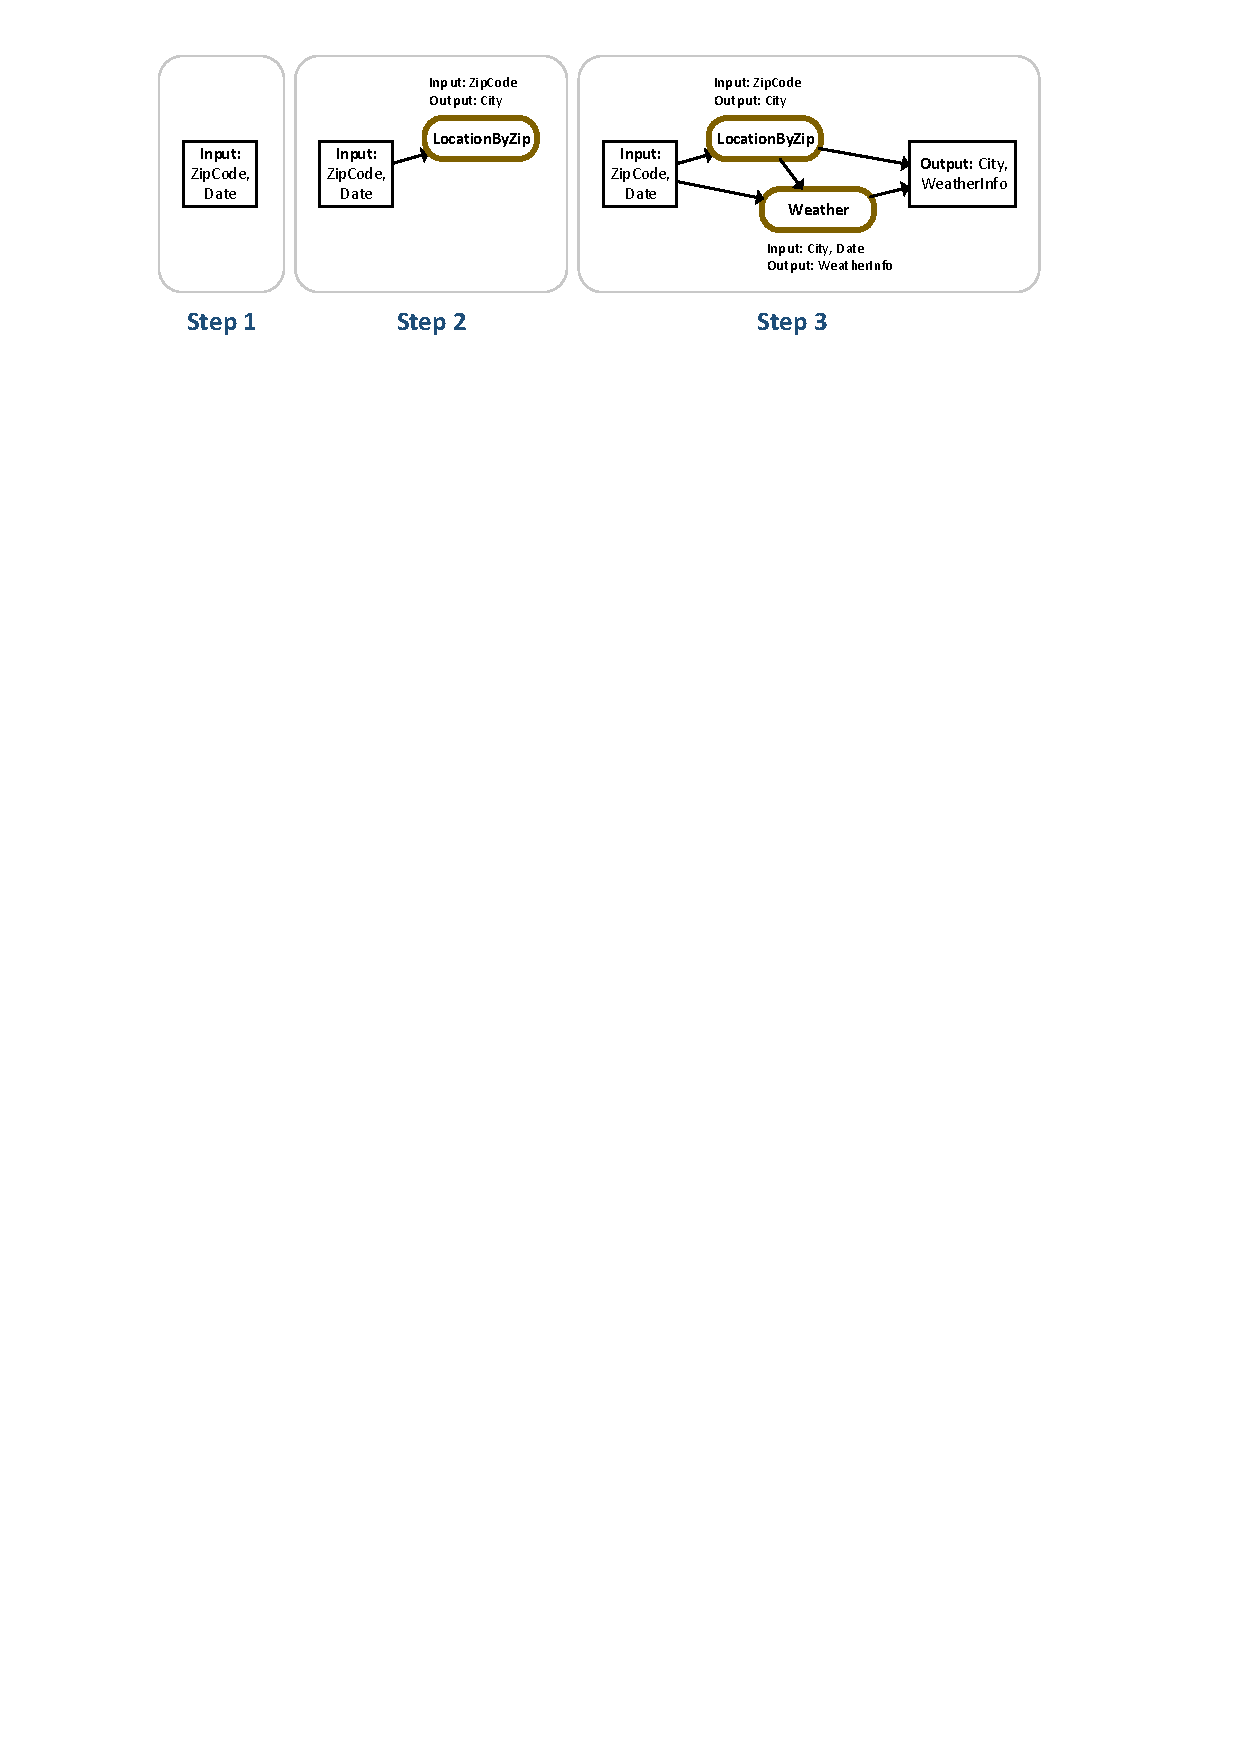
\includegraphics[width=14cm]{graphplan.pdf}
%}}
%\caption{Basic example of Web service composition using the Graphplan algorithm.}
%\label{fig:graphplan}
%\end{figure}

%In \cite{chen2014qos}, authors combine a planning algorithm and a graph search algorithm to achieve both QoS optimisation and feasibility in Web service compositions. The generic Graphplan algorithm first builds a representation of the search space as a planning graph, then finds a solution within this graph by traversing it backwards. This standard planning approach is modified to use Dijkstra's algorithm \cite{skiena1990dijkstra} when performing the backwards traversal, thus finding an optimised solution. The planning graph is extended to include labels associated with each proposition (i.e. each intermediate action between two vertices), where each label contains a layer number and associated execution costs. Dijkstra's algorithm is used to calculate the upcoming costs of each node in the graph. Then, a backtracking algorithm uses this information to determine the optimal solution.

%The work in \cite{deng2013efficient} proposes a planning-graph approach to creating a Web service composition technique that is capable of identifying the top K solutions with regards to overall QoS values. According to authors, AI planning is highly suitable to the domain of service composition, however many planning approaches are not efficiently executed. A notable exception to this trend is the planning-graph method, where the search space is greatly reduced through an initial search, thus allowing the remainder of the algorithm to focus on the relevant areas of the search space. In this work, the planning-graph approach is employed in a three-part algorithm. In the first part, a forward search is executed from the input node aiming to find the output node, gradually filtering the services that could be used in the composition. In the second part, the optimal local QoS of each service in the remaining graph is calculated using functions that take into consideration the QoS of the services that could possibly feed its input, also executed from the input node towards the output. Finally, a backward search algorithm is executed to generate the top K solutions according to local values calculated in the previous step (a threshold is provided when running this algorithm to prune out the substandard composition options).

%An automated Web service composition approach that uses a filtering algorithm to reduce the number of services considered for the composition, organising the remaining services as a graph according to the ways in which their inputs and outputs match, is proposed in \cite{huang2009effective}. Once the graph has been determined, a modified dynamic programming approach is applied to it in order to calculate the composition with the optimal QoS. Dynamic programming is a method that breaks problems into smaller subproblems that are then solved, ultimately leading to the solution of the parent problem. In this case, the optimal QoS of each atomic service in the graph is calculated, taking into account its input dependencies. At the end of this process, the overall optimal QoS values are known and the subgraph containing the solution can be extracted by searching the graph backwards. Experiments with the WSC2009 dataset show that the algorithm has good execution times for various dataset sizes, demonstrating its scalability. This work was extended in \cite{jiang2010qsynth}, with the presentation of a composition tool called QSynth, and the performance of formal comparisons with other state-of-the-art approaches, also producing superior results.

%A number of other works in the area employ formal AI planning techniques and frameworks to create compositions \cite{bertoli2009control}. The work in \cite{sohrabi2009web} presents an approach to include user preferences into the process of Web service composition. This is accomplished by relying on a framework written in Golog, a language created for agent programming. Golog is used to specify the particular attributes of generic workflows that represent commonly requested composition procedures (an example of a generic workflow would be one that is dedicated to booking inter-city transportation). The syntax of a logic-based language used to specify user preferences is described, allowing for branching according to conditions, and for expressing preferences over alternative services. Despite supporting branching, only one set of final outputs is allowed, meaning that the branches must be merged before reaching the end node of the composition workflow.

%An approach for modelling the data flow between Web services through the use of \textit{domain objects} is presented in \cite{kazhamiakin2013data}. For example, the travel domain contains objects such as flight ticket, hotel reservation, etc. The key idea is to use these objects to connect the composition needs to the services that can address them. In order to do so, authors annotate how each Web service operation relates to a given domain object. By creating this abstraction layer of objects, it is possible to reduce the composition's dependency on implementation details for correct execution. Now services can be thought of as having an object port proxy that leads to specific service ports. Compositions can then be achieved by identifying the necessary domain objects for the required task. The paper goes on to show how this technique can be integrated into existing service composition techniques, in this case AI-planning based, through the creation of a formal framework. This framework was implemented and run with a virtual travel agency scenario. According to the authors, the implementation of such framework was not trivial, however it successfully demonstrates that service implementations can be modified without impacting the overall composition.

%A Web service composition approach that allows users to specify constraints on the data flow of the solutions (i.e. which routes a message is allowed to take and which manipulations it can undergo) is presented in \cite{marconi2006specifying}. For example, consider a Web service composition that is supposed to book a holiday for a customer using a flights, accommodation, and a map service. If it is possible to book a suitable flight but it is not possible to book a hotel, the customer should not accept the offer. This is the type of requirement addressed by this approach using a data flow modelling language. This is a visual language that supports the definition of inputs/outputs, forking messages, merging messages, operations on messages, etc. By connecting these elements we obtain \textit{data nets} whose satisfiability can be clearly verified. The composition of Web services is performed using a planning framework that is capable of interpreting and respecting the constraints of a data net. At the time this paper was written, this approach had not yet been implemented or tested.

%\subsection{Hybrid Approaches}

%Hybrid approaches combine elements of AI planning and optimisation techniques for solving the composition problem with functionally correct, optimised solutions \cite{cotta2007memetic,pop2011tabu,xiang2011qos,chifu2012optimizing}. These hybrid approaches are quite similar to each other, relying on a directed acyclic graph as the base representation for a candidate solution, and then applying the optimisation techniques to this structure. However, despite incorporating the use of planning techniques, they do not include any discussion on the issue of producing solutions that satisfy conditional constraints or preferences. Another commonality between these works is that they require the use of SAWSDL-annotated datasets for testing, but these are not widely available to the research community. Therefore, authors developed their own datasets, and utilised each dataset's optimal task solution as the benchmark with which to evaluate the success of their implementation. More specifically, authors calculated the percentage of runs that culminated in the identification of the global optimum  as the recommended solution.

%In \cite{pop2010immune}, an approach that combines AI planning and an immune-inspired algorithm is used to perform fully automated QoS-aware Web service composition, also considering
%semantic properties. One significant contribution of this work is the proposal of an Enhanced Planning Graph (EPG), which extends the traditional planning graph structure
%by incorporating semantic information such as ontology concepts. Given this data structure, the composition algorithm selects the best solution configuration from a set of candidates. A fitness function considering QoS values and semantic quality is used to judge the best solution, and a clonal selection approach is employed to perform the optimisation. Candidates cells (solutions) are cloned, matured (mutated by replacing services with others from the same cluster in the EPG) and the cell most suited to combating the invading organism (i.e. the best solution) is discovered.

%The work in \cite{pop2011hybrid} proposes the employment of the Firefly meta-heuristic technique for performing QoS-aware Web service composition, in conjunction with an AI planning strategy that uses an EPG as the basis for solutions. The firefly meta-heuristic is based on the behaviour of mating fireflies, which emit a flashing light to attract potential mates. Each artificial firefly investigates the search space, with each position representing a composition solution. The brightness of the firefly is represented by the fitness of the current solution (location) associated with it. Fireflies are attracted to others according to their brightness, which varies with distance. Finally, fireflies move towards the individuals they are attracted to, meaning that small modifications occur in the current solution. The fitness function takes into account the QoS attributes of the composition.

%\section{Semantic Selection Approaches}\label{semantic}
%One important issue when creating compositions is that of selecting services that are compatible to each other. The simplest way of achieving this is by ensuring that the conceptual output and input types of any two services we wish to connect are perfectly matched, as illustrated by the Graphplan algorithm example in Section \ref{planning}. This involves accessing each service's WSDL, which is a formal description of a Web service's interface \cite{curbera2002unraveling}, and determining whether the two services offer compatible operations. However, in a more realistic scenario it may be very difficult to identify two services with such a precise fit. Because of this, an area of focus in the field of composition is that of semantic Web service selection. The fundamental idea of this approach is to annotate each service with additional semantic information so that the matching of services can be accomplished at a conceptual level. A well-known semantic standard for Web services is OWL-S (Web Ontology Language for Services) \cite{martin2007bringing} standard. OWL-S provides a formal specification of the workings of a service, allows for the association of conceptual classes with each Web service, and supports the use of ontologies that record the relationships between members of these different classes, thus establishing a common vocabulary for inter-service interactions. These features are conducive to automating the handling of Web services, and facilitating the discovery of those that are relevant for a specific task. Another more recent standard for semantic Web service annotation is SAWSDL (Semantic Annotations for WSDL) \cite{kopecky2007sawsdl}, a language that builds on WSDL by embedding pointers in the WSDL description that refer to semantic concepts. These pointers are called annotations, and are linked to concepts in a higher-level ontology layer.

%A number of different selection techniques that use semantic descriptions have been proposed recently \cite{soydan2004daml,wang2006qos,garcia2008qos,lin2008web,karakoc2009composing,boustil2010web,saboohi2011world,li2013towards,zhang2013genetic}. The work in \cite{DBLP:journals/soca/BoustilMS14}, for example, presents a selection strategy that considers more than just WSDL-level descriptions for Web services. In this approach, objects with additional information that is useful to the selection process are associated with each service. These objects have an independent ontology that describes how they interrelate (e.g. a service for making medical appointments has associated objects such as doctor, patient, hospital/clinic, etc), and at composition time the compatibility of these objects is verified. To accomplish this, a framework with service providers, ontology providers, information agents and a composer is proposed. This framework takes selection constraints set by the user into account.

%An automated semantic composition method is proposed in \cite{shin2007automated}. In this method, services are classified according to a functionality tag consisting of an \{action, object\} pair (e.g. a service for calculating the distance between two cities has the tag \{Calculate, Distance\}). A service relation graph is created to illustrate the dependencies between concepts, and it is divided in three parts: a graph showing relationships between actions, another graph showing relationships between objects (input/output relationships), and a mapping between items in these graphs. The relationships between these items are determined using domain ontology trees, with the assumption that these trees have already been provided. Given these dependencies, an algorithm is used to find a composition path. The path is found through the action graph and service connections are made based on the object graph, not only the object names. This approach was shown to require substantially less time to execute for larger datasets than previously proposed methods.

%The work in \cite{guo2010four} proposes a semantic Web service selection method that performs matching based on four distinct levels. At the \textit{Application Domain Matching} level the domain that best matches the user request is identified through the use of category ontologies, and a list of potential service description candidates is retrieved. This is performed by calculating a similarity degree between the user request and the semantic information associated with each domain. Subsequently, at the \textit{Service Description Matching} level, vectors are created for each potential service candidate description based on a given domain ontology, and another vector is created to represent the user requirements. A Vector Space Model is created, employing cosine similarity and TF-IDF to select the best service description. At the \textit{Service Function Matching} level, information from service providers is compared to the service description using a similarity measure, and a set of all services whose functionality fulfils the requirements is returned. Finally, at the \textit{QoS Matching} level, a matching array of quality values showing how closely a Web service matches the user's requirements is calculated, and the optimal candidate is returned.

%A framework for performing semantic Web service composition that also allows for user constraints to be specified is proposed in \cite{gamha2008framework}. Initially, services are grouped into distributed "service communities" according to their OWL-S semantic descriptions, where each community has services that cater for similar domains and consequently present similar functionalities. Then, users formulate their composition needs, including the necessary constraints, using terms from the semantic service community descriptions. Effectively, they create an abstract workflow for semi-automated composition by using the community descriptions and specifying their own preferences for the services to be selected. These constraints may be restrictions in input value ranges, in the output value ranges, or other service parameters. A language called KIF was chosen to express the constraints according to the corresponding OWL-S service descriptions. Interestingly, this approach can also handle world-altering services and non-deterministic functionality because it makes use of statecharts to model the behaviour of services.

%\section{Dynamic Web Service Composition}\label{dynamic}
%The approaches discussed thus far can be classified as static Web service composition, since they maintain a closed world assumption, that is, they assume that that the quality and the state of the services in the composition remains constant over time. However, in reality the state of the services available in a repository changes as time goes by, causing fluctuations in quality and even occasional failures. The area of dynamic Web service composition removes the closed world assumption, exploring solutions that can cope with quality fluctuations and service failures \cite{alferez2013facing,berg2013revenue,DBLP:journals/soca/WenTLCLH14}. The work in \cite{khakhkhar2012dynamic} proposes an algorithm that quickly creates a solution to satisfy a runtime service request, modelling the service composition problem as a graph in which a path is to be found. Forward and backward chaining approaches based on input/output matches are used for path exploration, relying on heuristics to encourage the exploration of the most promising paths and to reduce the number of services considered. In the approach proposed by this paper, both forward chaining and backward chaining are employed simultaneously, with the intention of having their paths meet in the middle. By doing so, the number of branches to be considered is greatly reduced. Experiments showed that the bidirectional search requires the exploration of a consistently smaller number of services when compared to the exclusively forward and exclusively backward approaches.

%A multi-objective Web service selection approach that optimises solutions according to two functions, a static one that calculates the overall quality of service (QoS) of a solution, and a dynamic one which calculates the \textit{trust degree} of a solution at a given time, is presented in \cite{wang2014novel}. The trust degree is defined as the number of successful executions of a service over its total number of executions, a piece of information that can be obtained by analysing execution logs. The optimisation algorithm used in this approach is an adaptive form of ant colony optimisation (ACO), where pheromones are adjusted according to the trust degree (calculated anew at every iteration) and the QoS is used by each ant as the heuristic for choosing the next node to visit. Each node in the graph explored by the ants represents an abstract service, with multiple concrete service candidates which can provide that functionality. The algorithm works by generating a set of of solutions and then identifying its Pareto subset by comparing all solutions. The Pareto subset is used in the next iteration, for updating the path pheromones. A case study is presented, comparing the performance of adaptive ACO to that of of the standard ACO algorithm, with results showing that adaptive ACO has a higher accuracy percentage than the standard ACO.

%The notion of transactions can be associated with service compositions, where different transactional properties guarantee certain runtime behaviours in a dynamic environment. The work in \cite{el2010tqos} proposes a semi-automated Web service composition approach that not only takes the functionality and quality of the services into account, but also their transactional properties. In this work, transaction properties are defined as the behaviour of Web services when interacting with one another. Knowing the behaviour of Web services is important for estimating how reliable their execution is and which ones might require recovery strategies at runtime. A service is considered \textit{retriable} if it can terminate successfully after multiple invocations, \textit{compensatable} if there is another service that can semantically undo its effects, and \textit{pivot} if its effects cannot be undone once it is executed but if it fails there are no effects. The system takes an abstract workflow and a set of user preferences as its inputs, where the user preferences contain QoS weights and risk levels corresponding to the transitional requirements for the composition. Then, a planner engine assigns one concrete Web service to each abstract slot of the provided workflow. Whenever a service is assigned to a part of the workflow, its transactional properties influence any subsequent services, thus the risk must be recalculated along with the overall QoS. Experiments were run for various risk scenarios, and computation time was found to remain under 2 seconds even for the largest dataset (comprising 3602 atomic Web services), at the same time meeting user preferences.

%An approach to QoS-aware Web service composition that is focused on \textit{rebinding}, that is, deciding which concrete services to bind to each abstract task at runtime in order to take the current state of the environment into consideration, is presented in \cite{parejo2014qos}. This approach considers global QoS constraints (e.g. the overall composition price must be lower than 5), local QoS constraints (e.g. the individual price for a service must be no higher than 1), and service dependency constraints (e.g. as many services as possible should be used from the same provider). Two techniques are employed during the composition process: GRASP, which is used to construct initial solutions, and Path Relinking, which is used to perform improvement on these solutions. \textit{GRASP} (Greedy Randomized Adaptive Search Procedure) iteratively builds a \textit{valid} solution vector, adding one candidate to fulfil each solution slot at a time and ensuring that this candidate respects the pre-established user constraints. The order of candidate addition matters, so it is performed randomly each time. Once a valid solution has been built, GRASP identifies a list of replacement candidates for each task slot, including the most promising candidates while also respecting the constraints observed by the valid solution. \textit{Path Relinking} explores the neighbouring solutions of the initial valid solution, seeking to further improve it. To do so, it slowly modifies solutions by changing services from one task slot at a time. The objective function used in this paper encourages the improvement of QoS values at the same time it enforces the relevant user constraints.

%\section{Summary and Limitations}\label{summary}
%This chapter presented an overview of the recent research conducted on different aspects of the automated Web service composition problem. The first area explored was that of \textbf{single-objective composition}, which aims to create composite solutions with the best possible overall Quality of Service (QoS) by conducting optimisations according to an objective function. Different approaches have been attempted for this, including both traditional approaches such as Integer Linear Programming (ILP) and Evolutionary Computation (EC) approaches such as Genetic Programming (GP), though in certain cases traditional approaches may not scale well as the composition problems grow in complexity. One key limitation of single-objective composition approaches is that they neglect the issue of branching, that is, they do not allow the creation of solutions with multiple alternative outputs that may be produced depending on a condition. To overcome this problem, a new candidate representation that also encodes this form of conditional branching needs to be proposed.

%Another area discussed is that of \textbf{multi-objective, top-K, and many-objective composition}, where each QoS attribute is optimised separately, and a set of solutions presenting trade-offs between these different quality attributes is generated. Multi-objective approaches work best for optimisation problems that involve two or three independent dimensions, while many-objective approaches are capable of handling more than three of them; top-K aims to produce a predetermined number of solution options based on a ranking strategy. The optimisation of multiple independent objectives is complex and provides many possibilities for further exploration. One interesting problem is that of many-objective optimisation for SLA-aware Web service composition, which refers to the constrained optimisation of several independent objectives to reflect the minimum quality requirements of the composition requestor. Accomplishing this is particularly challenging when creating solutions with multiple output possibilities.

%A number of \textbf{AI planning-based composition} approaches are also presented in this chapter. Their fundamental idea is to build solutions step by step, adding one atomic service to the composition at a time and subsequently checking whether the overall desired output has now been produced. These approaches are conducive to ensuring that the generated solutions are feasible and also included conditional branches into the solution's workflow whenever necessary. Despite these advantages, it is difficult to globally optimise the quality of a solution produced through planning, since its components are not modified or improved once they have been selected. A promising strategy to overcome this problem would be to combine planning algorithms with a population-based approach for optimisation, though this avenue has not yet been significantly explored by researchers.

%The \textbf{semantic Web service selection} approaches examined in this chapter propose a more realistic way of selecting the atomic components of a composition. Instead of expecting the return values and parameter types of service operations to match perfectly, the closest possible output-input matches are calculated using semantic distance measurements. The limitation of most works in this area is that they restrict their selection technique to semi-automated composition, where it is assumed that a framework with abstract service slots that are to be filled by concrete atomic services has already been provided. In the case of composition approaches based on AI planning techniques, where the workflow is built as services are connected to the solution, more flexible semantic selection methods are necessary. This motivates further research in this area.

%Finally, this chapter focuses on the issue of \textbf{dynamic Web service composition}. In this type of composition a closed world is abandoned, meaning that the state of services is expected to change throughout time. This brings two main problems: firstly, when the quality of the services in a repository changes, a solution that was once optimised according to the previous quality measures may suddenly transform into a low-standard alternative; secondly, certain services may become unavailable, meaning that solutions which incorporate them are henceforth unusable. The dynamic composition approaches discussed in this chapter use a variety of self-healing and recovery techniques to adjust solutions according to these changes, however they do not rely on EC techniques for doing so. These techniques can quickly re-optimise the QoS of existing solutions and provide composition backups (i.e. other candidates in the population) in case of failure, thus making EC an interesting dynamic alternative.
